\documentclass{beamer} %
\usetheme{CambridgeUS}
\usepackage[slovene]{babel}  % slovenščina
\usepackage[T1]{fontenc}     % naprednejše kodiranje fonta
\usefonttheme{professionalfonts}
\usepackage{times}
\usepackage{tikz}
\usepackage{amsmath}
\usepackage{verbatim}
\usetikzlibrary{arrows,shapes}

\author{Matic Oskar Hajšen in Eva Zmazek}
\title{Gibanja togih teles}

% ukazi za matematična okolja
\theoremstyle{definition} % tekst napisan pokončno
\newtheorem{definicija}{Definicija}[section]
\newtheorem{primer}[definicija]{Primer}
\newtheorem{opomba}[definicija]{Opomba}
\newtheorem{aksiom}{Aksiom}

\theoremstyle{plain} % tekst napisan poševno
\newtheorem{lema}[definicija]{Lema}
\newtheorem{izrek}[definicija]{Izrek}
\newtheorem{trditev}[definicija]{Trditev}
\newtheorem{posledica}[definicija]{Posledica}

\numberwithin{equation}{section}  % števec za enačbe zgleda kot (2.7) in se resetira v vsakem poglavju

% Matematični ukazi
\newcommand{\R}{\mathbb R}
\newcommand{\N}{\mathbb N}
\newcommand{\Z}{\mathbb Z}
%\renewcommand{\C}{\mathbb C}
\newcommand{\Q}{\mathbb Q}
\renewcommand{\H}{\mathbb H}

\begin{document}



\begin{frame}
\titlepage
\end{frame}

\begin{frame}
\frametitle{Homogene in kartezične koordinate}

$P$ vektor v $3$-dimenzionalnem prostoru $\R^3$\\

\begin{itemize}
\item Homogene koordinate vektorja $P$: $$p = (p_0,p_1,p_2,p_3)^T \in \R^4 / \{(0,0,0,0)^T\}$$
\item Če $p_0 \not= 0$, potem so kartezične koordinate vektorja $P$ enake $$\underline{p} = (\underline{p_1}, \underline{p_2}, \underline{p_3})^T \in \R^3;~  \underline{p_i} = \frac{p_i}{p_0} \text{ za } i=1,2,3$$
\item Vektorjem z ničelno prvo homogeno komponento priredimo točke v neskončnosti.
\end{itemize}

\begin{opomba}
Vektorja $p$ in $\lambda p$ v homogenih koordinatah opisujeta isti vektor $\underline{p}$ v kartezičnih koordinatah za poljubno neničelno realno število $\lambda$.
\end{opomba}

\end{frame}

\begin{frame}
\frametitle{Fiksen in gibajoč se koordinatni sistem}

Definirajmo dva koordinatna sistema v $\R^3$:
\begin{itemize}
\item fiksen koordinatni sistem $E^3$ (običajen koordinatni sistem)
\item gibajoč se koordinatni sistem $\hat{E}^3$
\end{itemize}
Točke lahko predstavimo v enem ali drugem.\\

\begin{figure}[h!]
\centering
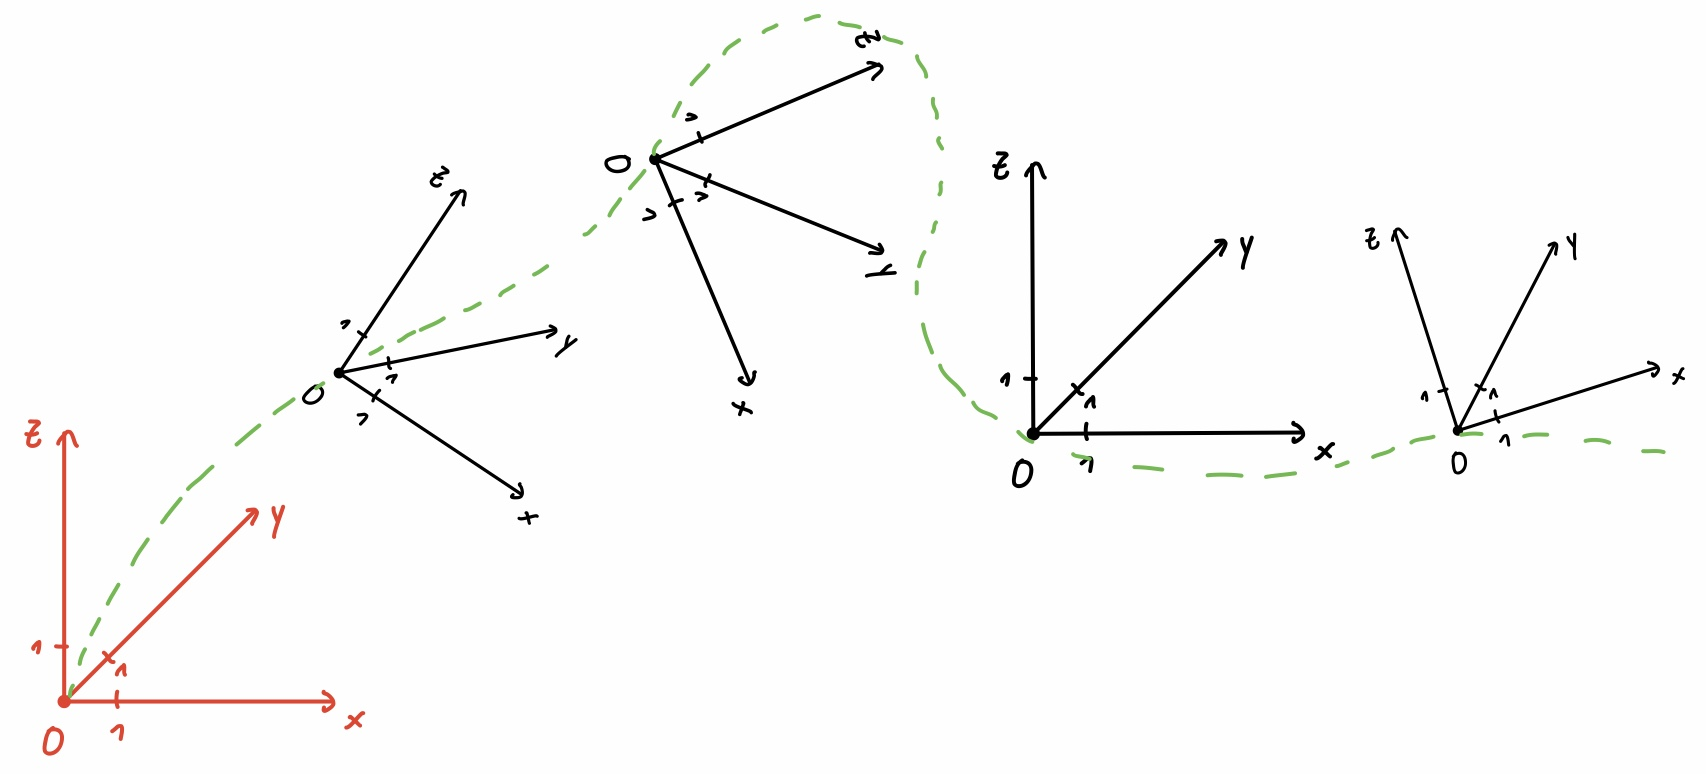
\includegraphics[width=0.75\textwidth]{koordinatnasistema}
\end{figure}

\end{frame}

\begin{frame}
Potrebujemo koordinatno transformacijo
$$\hat{E}^3 \to E^3$$
$$\hat{p} \mapsto p$$


$$M =
\left[
\begin{tabular}{c | c c c}
$m_{0,0}$ & $0$ & $0$ & $0$ \\
\hline
$m_{1,0}$ & $m_{1,1}$ & $m_{1,2}$ & $m_{1,3}$ \\
$m_{2,0}$ & $m_{2,1}$ & $m_{2,2}$ & $m_{2,3}$ \\
$m_{3,0}$ & $m_{3,1}$ & $m_{3,2}$ & $m_{3,3}$ \\
\end{tabular}
\right],
$$

$$\hat{p} \mapsto p = M \hat{p}$$

\end{frame}

\begin{frame}
\frametitle{Transformacija koordinatnega izhodišča}

Koordinatno izhodišče:
\begin{itemize}
\item v kartezičnih koordinatah: $(0,0,0)^T$
\item v homogenih koordinatah: $(1,0,0,0)^T$
\end{itemize}

\vspace{1cm}
Transformirano koordinatno izhodišče:
\begin{itemize}
\item v homogenih koordinatah:
$$c = M (1,0,0,0)^T = (m_{0,0}, m_{1,0}, m_{2,3}, m_{3,0})^T$$
\item v kartezičnih koordinatah:
$$\underline{c} = (\frac{m_{1,0}}{m_{0,0}}, \frac{m_{2,0}}{m_{0,0}}, \frac{m_{3,0}}{m_{0,0}})^T$$
\end{itemize}

\end{frame}

\begin{frame}
\frametitle{Rotacijska matrika}

$$\underline{R} =
\frac{1}{m_{0,0}}
\left[
\begin{tabular}{c c c}
$m_{1,1}$ & $m_{1,2}$ & $m_{1,3}$ \\
$m_{2,1}$ & $m_{2,2}$ & $m_{2,3}$ \\
$m_{3,1}$ & $m_{3,2}$ & $m_{3,3}$ \\
\end{tabular}
\right]
$$

\noindent opisuje orientacijo gibajočega se koordinatnega sistema $\hat{E}^3$
%\noindent $\underline{c}$ predstavlja položaj izhodišča koordinatnega sistema $\hat{E}^3$ v koordinatni sistem $E^3$, $R$ pa je \textbf{rotacijska matrika}, ki opisuje rotacijo gibajočega se koordinatnega sistema. \\

\end{frame}

\begin{frame}
\frametitle{Transformacija vektorja $[1,b_M,c_M,d_M]$}


$$d = 
M
\cdot
\left[
\begin{tabular}{c}
$1$ \\
$b_M$ \\
$c_M$ \\
$d_M$
\end{tabular}
\right]
=
\left[
\begin{tabular}{c}
$m_{0,0}$ \\
$m_{1,0}$ \\
$m_{2,0}$ \\
$m_{3,0}$ \\
\end{tabular}
\right]
+
\left[
\begin{tabular}{c c c}
$0$ & $0$ & $0$ \\
$m_{1,1} b_M$ & $m_{1,2} c_M$ & $m_{1,3} d_M$ \\
$m_{2,1} b_M$ & $m_{2,2} c_M$ & $m_{2,3} d_M$ \\
$m_{3,1} b_M$ & $m_{3,2} c_M$ & $m_{3,3} d_M$ \\
\end{tabular}
\right]
$$

$$d_0 = m_{0,0}$$
$$\left[
\begin{tabular}{c}
$d_1$ \\
$d_2$ \\
$d_3$ \\
\end{tabular}
\right]
=
\left[
\begin{tabular}{c}
$m_{1,0}$ \\
$m_{2,0}$ \\
$m_{3,0}$ \\
\end{tabular}
\right]
+
\left[
\begin{tabular}{c c c}
$m_{1,1}$ & $m_{1,2}$ & $m_{1,3}$ \\
$m_{2,1}$ & $m_{2,2}$ & $m_{2,3}$ \\
$m_{3,1}$ & $m_{3,2}$ & $m_{3,3}$ \\
\end{tabular}
\right]
\cdot
\left[
\begin{tabular}{c}
$b_M$ \\
$c_M$ \\
$d_M$
\end{tabular}
\right]
$$

\end{frame}

\begin{frame}


$$d_0 = m_{0,0}$$
$$\left[
\begin{tabular}{c}
$d_1$ \\
$d_2$ \\
$d_3$ \\
\end{tabular}
\right]
=
\left[
\begin{tabular}{c}
$m_{1,0}$ \\
$m_{2,0}$ \\
$m_{3,0}$ \\
\end{tabular}
\right]
+
\left[
\begin{tabular}{c c c}
$m_{1,1}$ & $m_{1,2}$ & $m_{1,3}$ \\
$m_{2,1}$ & $m_{2,2}$ & $m_{2,3}$ \\
$m_{3,1}$ & $m_{3,2}$ & $m_{3,3}$ \\
\end{tabular}
\right]
\cdot
\left[
\begin{tabular}{c}
$b_M$ \\
$c_M$ \\
$d_M$
\end{tabular}
\right]
$$

$$\underline{d}
=
\frac{1}{m_{0,0}}\left[
\begin{tabular}{c}
$m_{1,0}$ \\
$m_{2,0}$ \\
$m_{3,0}$ \\
\end{tabular}
\right]
+
\frac{1}{m_{0,0}}
\left[
\begin{tabular}{c c c}
$m_{1,1}$ & $m_{1,2}$ & $m_{1,3}$ \\
$m_{2,1}$ & $m_{2,2}$ & $m_{2,3}$ \\
$m_{3,1}$ & $m_{3,2}$ & $m_{3,3}$ \\
\end{tabular}
\right]
\cdot
\left[
\begin{tabular}{c}
$b_M$ \\
$c_M$ \\
$d_M$
\end{tabular}
\right]=
$$

$$=\underline{c} + R \cdot \underline{\hat{p}}$$

\noindent Transformacijo $\underline{\hat{p}} \mapsto \underline{p}$ v kartezičnih koordinatah zapišemo kot:
$$\underline{p} = \underline{c} + R \underline{\hat{p}}$$

\end{frame}

\begin{frame}
\frametitle{Gibanje točk v času}

\noindent Kadar je $\underline{c} = \underline{c}(t)$ in $R=R(t)$, govorimo o gibanju togega telesa:
$$\hat{E}^3 \times I \to E^3$$
$$(\underline{\hat{p}},t) \mapsto \underline{c}(t) + R(t) \underline{\hat{p}} =: \underline{p}(t)$$
Krivulji $\underline{p}(t)$ pravimo \textbf{trajektorija} točke $\underline{\hat{p}}$ \\

\begin{itemize}
\item Če je $c(t)=(0,0,0)^T$, se točka $\underline{\hat{p}}$ giblje po sferi z radije $||\underline{\hat{p}}||$
\item $R(t)$ se imenuje tudi \textbf{sferični del gibanja togega telesa}
\end{itemize}

\end{frame}

\begin{frame}
\frametitle{Opis rotacij s kvaternioni}
\begin{definicija}
Prostor kvaternionov $\H$ je $4$-dimenzionalni vektorski prostor s standardno bazo
$$ \underline{1} = (1, (0,0,0)^T) $$
$$ \underline{i} = (0,(1,0,0)^T) $$
$$ \underline{j} = (0,(0,1,0)^T) $$
$$ \underline{k} = (0,(0,0,1)^T) $$
\end{definicija}

\noindent Vsak kvaternion $\mathcal{A}$ lahko zapišemo kot:
$$\mathcal{A} = (a_0,\underline{a}),~ a_0 \in \R \text{ skalarni del },~ \underline{a} = (a_1,a_2,a_3)^T \text{ vektorski del}$$

\end{frame}

\begin{frame}
\frametitle{operacije na kvaternionih}

$$\mathcal{A} + \mathcal{B} = (a_0,\underline{a}) +(b_0,\underline{b}) = (a_0 + b_0,\underline{a} + \underline{b})$$
\vspace{0.5cm}
$$\mathcal{A} \cdot \mathcal{B}  = (a_0 \cdot b_0 - \underline{a} \cdot \underline{b}, a_0 \underline{b} + b_0 \underline{a} + \underline{a} \times \underline{b})$$
\vspace{0.5cm}
$$\overline{\mathcal{A}} = (a_0, - \underline{a})$$
\vspace{0.5cm}
$$|| \mathcal{A} || = \sqrt{\mathcal{A} \cdot \overline{\mathcal{A}}} = \sqrt{a_0^2 + a_1^2 + a_2^2 + a_3^2}$$

\end{frame}

\begin{frame}

\begin{definicija}
\label{definicijarotacije}
Preslikava $\chi : \H \backslash \{0\} \to SO_3$ oblike



$$Q  \mapsto \frac{1}{||Q||^2}
\left[
\begin{tabular}{c c c}
$q_0^2 + q_1^2 - q_2^2 - q_3^2$ & $2(q_1 q_2 - q_0 q_3)$ & $2(q_1 q_3 + q_0 q_2)$ \\
& & \\
$2(q_1 q_2 + q_0 q_3)$ & $q_0^2 - q_1^2 + q_2^2 - q_3^2$ & $2(q_2 q_3 - q_0 q_1)$ \\
& & \\
$2(q_1 q_3 - q_0 q_2)$ & $2(q_2 q_3 + q_0 q_2)$ & $q_0^2 - q_1^2 - q_2^2 + q_3^2$
\end{tabular}
\right]
$$

$$ Q = (q_0,(q_1,q_2,q_3)^T)$$
\\
se imenuje \textbf{kinematična preslikava}.
\end{definicija}

\end{frame}

\begin{frame}

\begin{itemize}
\item matrika $\chi(Q)$ je rotacijska matrika
\item vsako rotacijsko matriko $R$ lahko preslikamo v dva \textbf{antipodna kvaterniona} oblike
$$\pm Q = \pm(q_0,(q_1,q_2,q_3)^T),$$
$$q_0^2 + q_1^2 + q_2^2 + q_3^2 = 1$$
\end{itemize}

\end{frame}

\begin{frame}
\frametitle{Geometrijska interpretacija}
\noindent Vrednost $q_0$ in vektor $(q_1,q_2,q_3)^T$ lahko zato zapišemo v obliki:

$$q_0 = \cos(\frac{\phi}{2})$$

\vspace{0.5cm}

$$\left[
\begin{tabular}{c}
$q_1$ \\
$q_2$ \\
$q_3$
\end{tabular}
\right]
=
\sin(\frac{\phi}{2}) \cdot \vec{r}; ~ \vec{r} \text{ enotski vektor}
$$

\vspace{1cm}
\noindent Kvaternion $Q$ predstavlja rotacijo za kot $\phi$ okrog osi $\vec{r}$. \\

\end{frame}

\begin{frame}

\frametitle{Prirejanje kvaterniona podani matriki $M$}

\begin{align*}
m_{0,0} + m_{1,1} + m_{1,2} + m_{3,3} &= 4 q_0^2 \\
m_{3,2} - m_{2,3} = 2 \cdot (q_2 q_3 - q_0 q_1) - 2 \cdot (q_2 q_3 + q_0 q_1) &= 4 q_0 q_1 \\
m_{1,3} - m_{3,1} = 2 \cdot (q_1 q_3 + q_0 q_2) - 2 \cdot (q_1 q_3 + q_0 q_2) &= 4 q_0 q_2 \\
m_{2,1} - m_{1,2} = 2 \cdot (q_1 q_2 + q_0 q_4) - 2 \cdot (q_1 q_2 + q_0 q_4) &= 4 q_0 q_3 \\
& \\
m_{3,2} - m_{2,3} & = 4 q_0 q_1 \\
m_{0,0} + m_{1,1} - m_{1,2} - m_{3,3} &= 4 q_1^2 \\
m_{2,1} + m_{1,2} &= 4 q_1 q_2 \\
m_{1,3} + m_{3,1} &= 4 q_1 q_3 \\
\end{align*}

\end{frame}

\begin{frame}
\begin{align*}
m_{1,3} - m_{3,1} &= 4 q_0 q_2 \\
m_{2,1} + m_{1,2} &= 4 q_1 q_2 \\
m_{0,0} - m_{1,1} + m_{1,2} - m_{3,3} &= 4 q_2^2 \\
m_{3,2} + m_{2,3} &= 4 q_2 q_3 \\
& \\
m_{2,1} - m_{1,2} &= 4 q_0 q_3 \\
m_{1,3} + m_{3,1} &= 4 q_1 q_3 \\
m_{3,2} + m_{2,3} &= 4 q_2 q_3 \\
m_{0,0} - m_{1,1} - m_{1,2} + m_{3,3} &= 4 q_0^2 \\
\end{align*}

\noindent Razmerja:
$$ q_0 : q_1 : q_2 : q_3 $$

\end{frame}

\begin{frame}
\subsection{Bezierjeve krivulje}
\noindent Z uporabo kinematične preslikave lahko za konstrukcijo sferičnih gibanj uporabimo Bezierjeve krivulje. Izberemo kontrolne kvaternione $Q_0,Q_1,\dots,Q_n$.
$$Q(t) = \sum\limits_{i=0}^{n} Q_i B_i^n(t)$$
\noindent Bezierjeva krivulja $Q(t)$ v času $t$ opiše kvaternion, ki mu priredimo rotacijo $R(t)$:
$$\chi(Q(t)) = R(t)$$

\noindent Gibanje koordinatnega izhodišča zapišemo v obliki
$$\underline{c}(t) = \frac{w(t)}{||Q(t)||^2};~ w(t) := (w_1(t), w_2(t),w_3(t)).$$
($w(t)$ lahko podamo kot Bezierjevo krivuljo)

\end{frame}

\end{document}